\chapter{Functions}
\label{funcchap}

In the context of programming, a {\bf function} 
is usually a named sequence of statements 
that performs a computation.  In Perl, functions are often 
also called {\bf subroutines} and the two terms can (for now) 
be considered as more or less equivalent. When you define 
a function, you specify the name and the sequence of statements.  
Later, when you want to perform a computation, you can ``call'' 
the function by name and this will run the sequence of statements 
contained in the function definition.
\index{function}

Perl comes with many built-in functions that are quite handy.  
You've already seen some of them: for example, {\tt say} is a 
built-in function, and we will see many more in the course of 
this book. And if Perl doesn't already have a function that does 
what you want, you can build your own. This teaches you the basics 
of functions and how to build new ones.

\section{Function Calls}
\label{functionchap}
\index{function!call}

We have already seen examples of {\bf function calls}:

\begin{verbatim}
> say 42;
42
\end{verbatim}
%
The name of the function is {\tt say}.  The expression following 
the function name is called the {\bf argument} of the function. 
The {\tt say} function causes the argument to be displayed 
on the screen. If you need to pass several values to a function, 
then just separate the arguments with commas:
\begin{verbatim}
> say "The answer to the ultimate question is ", 42;
The answer to the ultimate question is 42
\end{verbatim}
%

Many programming languages require the arguments of a function to 
be inserted between parentheses. This is not required (and 
usually not recommended) in Perl~6 for most built-in functions 
(except when needed for precedence), but if you do use 
parentheses, you should make sure to avoid inserting spaces 
between the function name and the opening parenthesis. 
For example, the {\tt round} function usually takes two 
arguments: the value to be rounded and the unit or scale. 
You may call it in any of the following ways:

\begin{verbatim}
> round 42.45, 1;
42
> round 42.45, .1;
42.5
> round(42.45, .1);      # But not: round (42.45, .1);
42.5
> round( 42.45, .1);     # Space is OK *after* the opening paren
42.5
\end{verbatim}
\index{parentheses!argument in}

Experienced Perl programmers usually prefer to omit the parentheses 
when they can. Doing so makes it possible to chain several functions 
with a visually cleaner syntax. Consider for example the differences 
between these two calls:

\begin{verbatim}
> say round 42.45, 1;
42
> say(round(42.45, 1));
42
\end{verbatim}

The second statement is explicitly saying what is going on, but 
the accumulation of parentheses actually makes things 
not very clear. By contrast, the first statement can be seen 
as a pipeline to be read from right to left: the last function 
on the right, {\tt round}, is taking two arguments, 
{\tt 42.45, 1}, and the value produced by {\tt round} is 
passed as an argument to {\tt say}.

It is common to say that a function ``takes'' one or 
several arguments and ``returns'' a result.  The result is 
also called the {\bf return value}.
\index{argument}
\index{return!value}

Perl provides functions that convert values from one type 
to another.  When called with only one argument, the 
{\tt round} function takes any value and converts it to an 
integer, if it can, or complains otherwise:
\index{conversion!type}
\index{type!conversion}
\index{round function}
\index{function!round}

\begin{verbatim}
> round 42.3;
42
> round "yes"
Cannot convert string to number: base-10 number must begin with valid 
digits or '.' in '<HERE>yes' (indicated by <HERE>)
  in block <unit> at <unknown file> line 1
\end{verbatim}

%
Note that, in Perl~6, many built-in functions can also 
use a \emph{method invocation} syntax with the so-called 
dot notation. The following statements display the same result:
\index{invocation!method}
\index{method invocation}
\begin{verbatim}
> round 42.7;    # Function call syntax
43
> 42.7.round;    # Method invocation syntax
43
\end{verbatim}
%
The {\tt round} function can round off rational and 
floating-point values to integers. There is an {\tt Int} 
method that can also convert noninteger numerical values 
into integers, but it doesn't round off; it chops off the 
fraction part:
\index{Int method}
\index{method!Int}

\begin{verbatim}
> round 42.7
43
> 42.7.Int
42
\end{verbatim}

We'll come back to methods in the next section.

The {\tt Rat} built-in function converts integers and 
strings to rational numbers (if possible):
\index{Rat function}
\index{function!Rat}

\begin{verbatim}
> say 4.Rat;
4
> say 4.Rat.WHAT;
(Rat)
> say Rat(4).WHAT
(Rat)
> say Rat(4).nude
(4 1)
> say Rat('3.14159')
3.14159
> say Rat('3.14159').nude
(314159 100000)
\end{verbatim}
%
Finally, {\tt Str} converts its argument to a string:
\index{Str function}
\index{function!Str}

\begin{verbatim}
> say 42.Str.WHAT
(Str)
> say Str(42).WHAT;
(Str)
\end{verbatim}

\index{coercion}
\index{type!coercion}
Note that these type conversion functions often don't need 
to be called explicitly, as Perl will in many cases try to do the 
right thing for you. For example, if you have a string 
that looks like an integer number, Perl will \emph{coerce} 
the string to an integer for you if you try to apply 
an arithmetic operation on it:

\begin{verbatim}
> say "21" * "2";
42
\end{verbatim}

Similarly, integers will be coerced to strings if you 
apply the string concatenation operator to them:

\begin{verbatim}
> say 4 ~ 2;
42
> say (4 ~ 2).WHAT;
(Str)
\end{verbatim}

The coercion can even happen twice within the same expression 
if needed:

\begin{verbatim}
> say (4 ~ 1) + 1;
42
> say ((4 ~ 1) + 1).WHAT;
(Int)
\end{verbatim}

\section{Functions and Methods}
\index{function}
\index{method}

A method is similar to a function---it takes arguments and
returns a value---but the calling syntax is different. With 
a function, you specify the name of the function followed 
by its arguments. A method, by contrast, uses the dot 
notation: you specify the name of the object on which 
the method is called, followed by a dot and the name of 
the method (and possibly additional arguments).

A method call is often called an {\bf invocation}
\index{invocation}. The deeper differences between functions and
methods will become apparent much later, when studying 
object-oriented programming (in Chapter~\ref{objects}).
\index{invocation!method}
\index{method invocation}

For the time being, we can consider that the difference is 
essentially a matter of a different calling syntax when using Perl's 
built-ins. Most of Perl built-ins accept both a function 
call syntax and a method invocation syntax. For example, 
the following statements are equivalent:

\begin{verbatim}
> say 42;              # function call syntax
42
> 42.say;              # method invocation syntax
42
\end{verbatim}
%

You can also chain built-in routines with both syntactic 
forms:

\begin{verbatim}
> 42.WHAT.say;         # method syntax
(Int)
> say WHAT 42;         # function syntax
(Int)
> say 42.WHAT;         # mixed syntax
(Int)
\end{verbatim}
%

It is up to you to decide whether you prefer one form or the 
other, but we will use both forms, if only to get you used to 
both of them.

\section{Math functions}
\index{math function}
\index{function!math}

Perl provides most of the familiar mathematical functions.

For some less common functions, you might need to use a 
specialized module such as \verb'Math::Matrix' or 
\verb'Math::Trig'.  A {\bf module} is a file that contains a
collection of related functions.
\index{module}

Before we can use the functions in a module, we have to import it with
a {\bf use statement}:

\begin{verbatim}
use Math::Trig;
\end{verbatim}
%
This statement will import a number of functions that you will then be able to use as if you had defined them in your main source file, for example \verb'deg2rad' to perform conversion of angular values from degrees to radians, or \verb'rad2deg' to perform the opposite conversion.

For most common mathematical functions, however, you don't need any \verb'math' module, as they are included in the core of the language:

\begin{verbatim}
> my $noise-power = 5.5;
5.5
> my $signal-power = 125.6;
125.6
> my $decibels = 10 * log10 $signal-power / $noise-power;
13.5862694990693
\end{verbatim}
%
\index{log10 function}
\index{function!log10}
This first example uses \verb"log10" (common logarithm) 
to compute a signal-to-noise ratio in decibels 
(assuming that \verb"signal-power" and
\verb"noise-power" are defined in the proper units).  Perl 
also provides a {\tt log} function which, when receiving 
one argument, computes logarithm base {\tt e} of the argument, 
and, when receiving two arguments, computes the logarithm 
of the first argument to the base of the second argument:

\begin{verbatim}
> say e;                 # e is predefined as Euler's constant
2.71828182845905
> my $val = e ** e;
15.1542622414793
> say log $val;          # natural logarithm
2.71828182845905
> say log $val, e;       # logarithm base e or natural logarithm
2.71828182845905
> say log 1024, 2;       # binary logarithm or logarithm base 2
10
\end{verbatim}
%
\index{log function}
\index{function!log}


Perl also provides most common trigonometric functions:

\begin{verbatim}
> my $radians = 0.7;
0.7
> my $height = sin $radians;
0.644217687237691
\end{verbatim}

\index{sin function}
\index{radian}
\index{trigonometric function}
\index{function!trigonometric}
This example finds the sine of \verb'$radians'.  The name of the
variable is a hint that {\tt sin} and the other trigonometric
functions ({\tt cos}, {\tt tan}, etc.)  take arguments 
in radians. To convert from degrees to radians, you may 
use the  \verb'deg2rad' function of the 
\verb'Math::Trig module', or simply divide by 180 
and multiply by $\pi$:

\begin{verbatim}
> my $degrees = 45;
45
> my $radians = $degrees / 180.0 * pi;    # pi, predefined constant
0.785398163397448
> say sin $radians;       # should be square root of 2 divided by 2
0.707106781186547
\end{verbatim}
%
The expression {\tt pi} is a predefined constant for an
approximation of $\pi$, accurate to about 14 digits.
\index{pi}

If you know
trigonometry, you can check the previous result by comparing it to
the square root of two divided by two:
\index{sqrt function}
\index{function!sqrt}

\begin{verbatim}
> say sqrt(2) / 2;
0.707106781186548
\end{verbatim}
%

\section{Composition}
\index{composition}

So far, we have looked at the elements of a program---variables,
expressions, and statements---in isolation, without talking about how to combine them.

One of the most useful features of programming languages is their
ability to take small building blocks and {\bf compose} them, i.e., 
to combine them in such a way that the result of one is the 
input of another one.  For example, the argument of a function 
can be any kind of expression, including arithmetic operators:

\begin{verbatim}
> my $degrees = 45;
45
> my $height = sin($degrees / 360.0 * 2 * pi);
0.707106781186547
\end{verbatim}
%
Here, we have used parentheses for the argument to the {\tt sin} 
function to clarify that all the arithmetic operations 
within the parentheses are completed before the {\tt sin} function 
is actually called, so that it will use the result of these operations 
as its argument. 

You can also compose function calls:

\begin{verbatim}
> my $x = 10;
10
>  $x = exp log($x+1)
11
\end{verbatim}
%
Almost anywhere you can put a value, you can put an arbitrary
expression, with one exception: the left side of an assignment
statement has to be a variable name, possibly along with its
declaration.  Almost any other expression on the left
side is a syntax error \footnote{We will see rare exceptions to this rule
later}:

\begin{verbatim}
> my $hours = 1;
1
> my $minutes = 0;
0
> $minutes = $hours * 60;        # right 
60
> $hours * 60 = $minutes;        # wrong !!
Cannot modify an immutable Int
  in block <unit> at <unknown file> line 1
\end{verbatim}
%
\index{syntax error}


\section{Adding New Functions (a.k.a. Subroutines)}

\index{subroutine}
So far, we have only been using the functions that come with Perl,
but it is also possible to add new functions. In Perl, user-
defined functions are often called subroutines, but you might choose 
either word for them. 

A {\bf function definition} starts with the {\tt sub} keyword (for
subroutine) and specifies the name of a new subroutine and
the sequence of statements that run when the function is called.
\index{function}
\index{function!definition}
\index{definition!function}
\index{sub}

Here is an example of a subroutine quoting Martin Luther King's 
famous "I Have a Dream" speech at the Lincoln Memorial in 
Washington (1963):

\begin{verbatim}
sub print-speech() {
    say "Let freedom ring from the prodigious hilltops of New Hampshire.";
    say "Let freedom ring from the mighty mountains of New York.";
}
\end{verbatim}
%
{\tt sub} is a keyword that indicates that this is a subroutine
definition.  The name of the function is \verb"print-speech".  The
rules for subroutine names are the same as for variable names: letters,
numbers, and underscores are legal, as well as a dash or an 
apostrophe between letters, but the first character
must be a letter or an underscore.  You shouldn't use a 
language keyword (such as {\tt if} or {\tt while}) as 
the name of a function (in some cases, it might actually work, 
but it would be very confusing, at least for the human reader).
\index{sub!keyword}
\index{keyword!sub}
\index{argument}

The empty parentheses after the name indicate that this function
doesn't take any arguments. They are optional in that case, but are 
required when parameters need to be defined for the subroutine.
\index{parentheses!empty}
\index{header}
\index{body}

\index{indentation}
The first line of the subroutine definition is sometimes called 
the {\bf header}; the rest is called the {\bf body}.  The body 
has to be a code block placed between curly braces and it can contain
any number of statements. Although there is no requirement to do 
so, it is good practice (and highly recommended) to indent body 
statements by a few leading spaces, since it makes it easier to 
figure out visually where the function body starts and ends.
\index{curly bracket}
\index{curly brace}
\index{bracket!curly}


Please note that you cannot use a method-invocation syntax 
for subroutines (such as \verb"print-speech") that you write: 
you must call them with a function call syntax.
\index{method!invocation}
\index{function!call}
\index{invocation!method}
\index{method invocation}

The strings in the print statements are enclosed in double
quotes.  In this specific case, single quotes could have been 
used instead to do the same thing, but there are many cases 
where they wouldn't do the same thing, so you'll have to 
choose one or the other depending on the circumstances.
\index{double quote}
\index{quote!double}
\index{single quote}
\index{quote!single}


Most people use double quotes in cases where a single 
quote (which is also an apostrophe) appears in the string:
\index{apostrophe}
\begin{verbatim}
say "And so we've come here today to dramatize a shameful condition.";
\end{verbatim}
%
Conversely, you might use single quotes when double quotes 
appear in the string:
\begin{verbatim}
say 'America has given the Negro people a bad check, 
     a check which has come back marked "insufficient funds."';
\end{verbatim}
%
There is, however, a more important difference between single quotes 
and double quotes: double quotes allow variable interpolation, and 
single quotes don't.  Variable interpolation means that if a 
variable name appears within the double-quoted string, this 
variable name will be replaced by the variable value; within a 
single-quoted string, the variable name will appear verbatim. 
For example:
%
\begin{verbatim}
my $var = 42;
say "His age is $var.";            # -> His age is 42.
say 'Her age is $var.';            # -> Her age is $var.
\end{verbatim}
\index{interpolation}
\index{variable!interpolation}
%
The reason is not that the lady's age should be kept secret. 
In the first string, \verb'$var' is simply replaced within the 
string by its value, 42, because the string is quoted with double 
quotes; in the second string, \verb'$var' isn't replaced by 
its value because single 
quotes are meant to provide a more verbatim type of quoting 
mechanism. There are other quoting constructs offering finer 
control over the way variables and special characters are 
displayed in the output, but simple and double quotes are the most 
useful ones.

The syntax for calling the new subroutine is the same as
for built-in functions:

\begin{verbatim}
> print-speech();
Let freedom ring from the prodigious hilltops of New Hampshire.
Let freedom ring from the mighty mountains of New York.
\end{verbatim}
%

However, you cannot use the method-invocation syntax with 
such subroutines. We will see much later in this book (see 
Chapter~\ref{objects}) how to create methods. For the time 
being, we'll stick to the function-call syntax.
\index{invocation!method}
\index{method invocation}

Once you have defined a subroutine, you can use it inside another
subroutine.  For example, to repeat the previous excerpts of
King's address ,  we could write a subroutine called \verb"repeat_speech":

\begin{verbatim}
sub repeat-speech() {
    print-speech();
    print-speech();
}
\end{verbatim}
%
And then call \verb"repeat-speech":

\begin{verbatim}
> repeat-speech();
Let freedom ring from the prodigious hilltops of New Hampshire.
Let freedom ring from the mighty mountains of New York.
Let freedom ring from the prodigious hilltops of New Hampshire.
Let freedom ring from the mighty mountains of New York.
\end{verbatim}
%
But that's not really how the speech goes.


\section{Definitions and Uses}
\index{function!definition}

Pulling together the code fragments from the previous section, the
whole program looks like this:

\begin{verbatim}
sub print-speech () {
    say "let freedom ring from the prodigious hilltops of New Hampshire.";
    say "Let freedom ring from the mighty mountains of New York.";
}
sub repeat-speech () {
    print-speech();
    print-speech();
}
repeat-speech();
\end{verbatim}
%
This program contains two subroutine definitions: \verb"print-speech" and
\verb"repeat-speech".  Function definitions get executed just like other
statements, but the effect is to create the function.  The statements
inside the function do not run until the function is called, and
the function definition generates no output.

You don't have to create a subroutine before you can run it, 
the function definition may come after its call:
\begin{verbatim}
repeat-speech;
sub repeat-speech() {
    print_speech;
    print_speech;
}
sub print-speech() {
    # ...
}
\end{verbatim}


\section{Flow of Execution}
\index{flow of execution}

To ensure, for example, that a variable is defined (i.e., populated) 
before its first use, you have to know the order statements run in, 
which is called the {\bf flow of execution}.

Execution always begins at the first statement of the program 
(well, really \emph{almost} always, but let's say always 
for the time being). Statements are run one at a time, 
in order from top to bottom.

Subroutine definitions do not alter the flow of execution of the
program, but remember that statements inside a function don't
run until the function is called.

A function call is like a detour in the flow of execution. Instead of
going to the next statement, the flow jumps to the body of
the function, runs the statements there, and then comes back
to pick up where it left off.

That sounds simple enough, until you remember that one function can
call another.  While in the middle of one function, the program might
have to run the statements in another function.  Then, while
running that new function, the program might have to run yet
another function!

Fortunately, Perl is good at keeping track of where it is, so each
time a function completes, the program picks up where it left off in
the code that called it.  When it gets to the end of the program,
it terminates.

In summary, when you read a program, you
don't always want to read from top to bottom.  Sometimes it makes
more sense if you follow the flow of execution.


\section{Parameters and Arguments}
\label{parameters}
\index{parameter}
\index{function!parameter}
\index{argument}
\index{function!argument}

Some of the functions we have seen require arguments.  For
example, when you call {\tt sin} you pass a number
as an argument.  Some functions take more than one argument:
for example the {\tt round} function seen at the beginning 
of this chapter took two, the number to be rounded and 
the scale (although the {\tt round} function may accept a single argument, in which case the scale is defaulted to 1).

Inside the subroutine, the arguments are assigned to
variables called {\bf parameters}.  Here is a definition for
a subroutine that takes a single argument:
\index{parentheses!parameters in}

\begin{verbatim}
sub print-twice($value) {
    say $value;
    say $value
}
\end{verbatim}
%
This subroutine assigns the argument to a parameter
named \verb"$value". Another common way to say it is 
that the subroutine binds the parameter defined in its 
header to the argument with which it was called. When the 
above subroutine is called, it prints the content of the 
parameter (whatever it is) twice.

This function works with any argument value that can be printed:

\begin{verbatim}
> print-twice("Let freedom ring")
Let freedom ring
Let freedom ring
> print-twice(42)
42
42
> print-twice(pi)
3.14159265358979
3.14159265358979
\end{verbatim}
%
The same rules of composition that apply to built-in functions also
apply to programmer-defined subroutines, so we can use any kind of expression
as an argument for \verb"print-twice":
\index{composition}
\index{programmer-defined function}
\index{function!programmer defined}

\begin{verbatim}
> print-twice('Let freedom ring! ' x 2)
Let freedom ring! Let freedom ring! 
Let freedom ring! Let freedom ring! 
> print-twice(cos pi)
-1
-1
\end{verbatim}
%
The argument is evaluated before the function is called, so
in the examples the expressions \verb"'Let freedom ring! ' x 2" 
and {\tt cos pi} are only evaluated once.
\index{argument}

You can also use a variable as an argument:

\begin{verbatim}
> my $declaration = 'When in the Course of human events, ...'
> print-twice($declaration)
When in the Course of human events, ...
When in the Course of human events, ...
\end{verbatim}
%
The name of the variable we pass as an argument (\verb"$declaration") 
has nothing to do with the name of the parameter (\verb"$value"). It
doesn't matter what the variable was called back home (in the caller);
here, within \verb"print-twice", we call the parameter \verb"$value", 
irrespective of the name or content of the argument passed to the 
subroutine.


\section{Variables and Parameters Are Local}
\index{local variable}
\index{variable!local}
\index{scope}
\index{my}
\index{lexical scope}
\label{localvar}

When you create a variable inside a subroutine with the 
{\tt my} keyword, it is {\bf local}, or, more accurately, 
\emph{lexically scoped}, to the function block, which means 
that it only exists inside the function.  For example:
\index{parentheses!parameters in}

\begin{verbatim}
sub concat_twice($part1, $part2) {
    my $concatenation = $part1 ~ $part2;
    print-twice($concatenation)
}
\end{verbatim}
%
This function takes two arguments, concatenates them, and prints
the result twice.  Here is an example that uses it:
\index{concatenation}

\begin{verbatim}
> my $start = 'Let freedom ring from ';
> my $end = 'the mighty mountains of New York.';
> concat_twice($start, $end);
Let freedom ring from the mighty mountains of New York.
Let freedom ring from the mighty mountains of New York.
\end{verbatim}
%
When \verb"concat_twice" terminates, the variable \verb"$concatenation" 
is destroyed.  If we try to print it, we get an exception:
\index{Variable ... is not declared}
\index{exception!not declared}

\begin{verbatim}
> say $concatenation;
===SORRY!=== Error while compiling <unknown file>
Variable '$concatenation' is not declared
at <unknown file>:1
------> say <HERE>$concatenation;
\end{verbatim}
%
Parameters are also scoped to the subroutine.
For example, outside \verb"print-twice", there is no
such thing as \verb"$value".
\index{parameter}
\index{scope}


\section{Stack Diagrams}
\label{stackdiagram}
\index{stack diagram}
\index{function!frame}
\index{frame}

To keep track of which variables can be used where, it is sometimes
useful to draw a {\bf stack diagram}.  Like state diagrams, stack
diagrams show the value of each variable, but they also show the
function each variable belongs to.
\index{stack diagram}
\index{diagram!stack}

Each function is represented graphically by a {\bf frame}.  A frame 
is a box with the name of a function beside it and the parameters 
and variables of the function inside it.  The stack diagram for 
the previous example is shown in Figure~\ref{fig.stack}.

\begin{figure}
\centerline
{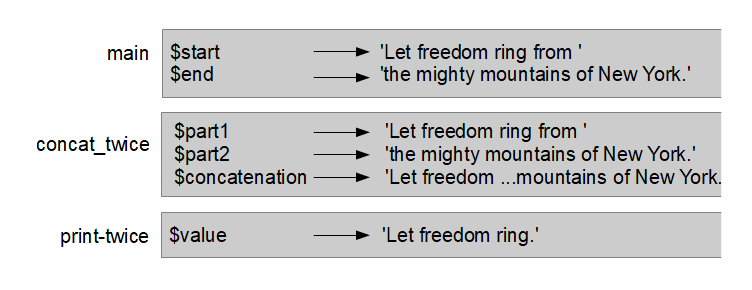
\includegraphics[scale=1.2]{figs/stack_diagram.png}}
\caption{Stack diagram.}
\label{fig.stack}
\end{figure}


The frames are arranged in a stack that indicates which function
called which, and so on.  In this example, \verb"print-twice"
was called by \verb"cat_twice", and \verb"cat_twice" was called by 
\verb"main", which is a special name for the topmost frame.  When
you create a variable outside of any function, it belongs to 
\verb"main".

Each parameter refers to the same value as its corresponding
argument.  So, {\tt \$part1} has the same value as
{\tt start}, {\tt \$part2} has the same value as {\tt \$end},
and {\tt \$value} has the same value as {\tt \$cat}.


\section{Fruitful Functions and Void Functions}
\index{fruitful function}
\index{void function}
\index{function, fruitful}
\index{function, void} 

Some of the functions we have used, such as the 
math functions, return results and are useful only insofar 
we use that return value; for lack of a better name, we 
may call them {\bf fruitful functions}.  Other functions, 
like \verb"print-twice", perform an action but don't appear 
to return a value (it does in fact return a value, {\tt True}, 
but we don't care about it).  They are sometimes called empty or 
{\bf void functions} in some other programming languages.

In some programming languages, such as Pascal or Ada, there 
is a strong distinction between a \emph{function} (which 
returns a value) and a \emph{procedure} (which doesn't); 
they are even defined with different keywords. This 
distinction does not apply to Perl and to most modern 
programming languages.

In fact, from a pure syntactic standpoint, Perl functions 
always return a result. So the distinction between 
``fruitful'' and ``void'' functions does not really exist 
syntactically, but only semantically, i.e., from the 
standpoint of the meaning of the program: maybe we need to 
use the return value, or maybe we don't.

Another distinction commonly made is between functions and 
mutators: functions do not change the initial state of the 
arguments they were called on, and mutators do modify it. We 
will not use this distinction here, but it is useful to 
keep it in mind.

When you call a fruitful function, you almost always
want to do something with the result; for example, you might
assign it to a variable or use it as part of an expression:

\begin{verbatim}
my $height = sin $radians;
my $golden = (sqrt(5) + 1) / 2;
\end{verbatim}
%
When you call a function in interactive mode (under the 
REPL), Perl usually displays the result:

\begin{verbatim}
> sqrt 5;
2.23606797749979
\end{verbatim}
%
But in a script, if you call a fruitful function all by 
itself, the return value is lost forever! In some cases, the 
compiler will be able to warn you, but not always. For example, 
consider the following program:

\begin{verbatim}
my $five = 5;
sqrt $five;
say $five;
\end{verbatim}

It produces the following warning:

\begin{verbatim}
WARNINGS for /home/Laurent/perl6_tests/sqrt.pl6:
Useless use of "sqrt $five" in expression "sqrt $five" in sink context (line 2)
5
\end{verbatim}
%
This script computes the square root of 5, but since 
it doesn't store or display the result, it is not very useful.
\index{interactive mode}
\index{script mode}

Void functions might display something on the screen, 
save some data to a file, modify a variable or an object, 
or have some other effect, but they generally don't have 
a return value, or at least not a useful one.  If you assign 
the result to a variable, you may get the return value of 
the subroutine, the value of the last expression which was 
evaluated in the function, or a special value such as 
{\tt Any}, which essentially means something that has not 
been defined, or {\tt Nil}.
\index{Any special value}
\index{special value!Any}
%

The subroutines we have written so far were essentially 
printing things to the screen. In that case, they 
usually return {\tt True}, at least when the printing 
was successful. Although they return a true value, what they 
return isn't very useful and we can consider them all void 
for our practical purposes.  

The following is an example of a very simple fruitful subroutine:
\index{return}

\begin{verbatim}
> sub square($number) { return $number ** 2 }
sub square ($number) { #`(Sub|118134416) ... }
> say square 5;
25
\end{verbatim}

The \verb'Sub|118134416' message displayed by the REPL is 
just an internal identifier for the subroutine we've just 
defined.

The {\tt return} statement instructs the function to terminate 
the execution of the function at this statement and to return 
the value of the following expression to the caller. In such a simple 
case where the program is in fact running the last statement 
of a function, the return keyword can be omitted since the function 
will return the value of the last evaluated statement, so that the 
{\tt square} subroutine could be written this way:
\begin{verbatim}
sub square($number) { 
    $number ** 2 
}
\end{verbatim}

We will be using fruitful functions more intensively in a 
few chapters.

\section{Function Signatures}
\index{function!signature}
\index{signature}

When a function receives arguments, which are stored into 
parameters, the part of the function 
definition describing the parameters between parentheses 
is called the {\bf function signature}. The function signatures 
we have seen so far are very simple and consist only of one 
parameter or possibly a parameter list.

Signatures can provide a lot more information about the 
parameters used by a function. First, you may define the 
type of the parameters. Some functions make sense only if their 
parameters are numeric and should probably raise an error if 
they get a string that cannot be converted to a numeric value. 
For example, if you define a function {\tt half} that computes 
a value equal to its argument divided by 2, it does not make 
sense to try to compute half of a string that is not numeric. 
It could be written as follows:
\index{type!parameter}
\index{parameter type}

\begin{verbatim}
sub half(Int $number) { 
    return $number / 2 
}
say half 84; # -> 42
\end{verbatim}

If this function is called with a string, we get the 
following error:
\index{type!String}

\begin{verbatim}
> say half "Douglas Adams"
===SORRY!=== Error while compiling <unknown file>
Calling half(Str) will never work with declared signature (Int $number)
at <unknown file>:1
------> say <HERE>half "Douglas Adams"
\end{verbatim}

The {\tt Int} type included in the function signature is a type 
constraint that can help prevent subtle bugs. In some cases, 
it can also be an annoyance. Consider this code snippet:
\index{constraint!type}
\index{type!constraint}
\index{type!Int}
\index{signature}


\begin{verbatim}
sub half(Int $number) {  $number / 2 }
say half "84"; # -> ERROR
\end{verbatim}

Because the argument to the {\tt half} subroutine is {\tt "84"}, 
i.e., a string, this code will fail with a type error. If we had 
not included the {\tt Int} type in the signature, the script 
would have converted (or \emph{coerced}) the "84" string to 
a number, divided it by two, and printed out the expected result:
\index{type!String}
\index{type!coercion}
\index{coercion!type}

\begin{verbatim}
sub half( $number) { $number / 2 }
say half "84"; # -> 42
\end{verbatim}

In some cases, you want this conversion to occur, in others 
you don't. It is up to you to decide whether you want 
strict typing or not, depending on the specific situation and
needs. It is probably helpful to use parameter typing in many 
cases, but it can also become a straitjacket in some situations. 
Perl~6 lets you decide how strict you want to be about these things.

Our original {\tt half} subroutine has another limitation: it
can work only on integers. But a function halving its argument 
should presumably be useful for rational or even other numbers. 
You can use the {\tt Real} or {\tt Numeric} types to make 
the function more general (the difference between the two 
types is that the {\tt Numeric} type will accept not only 
{\tt Real} but also {\tt Complex} numbers). As it turns out 
that this {\tt half} function will also work correctly 
with complex numbers, choosing a {\tt Numeric} 
type opens more possibilities:
\index{Numeric type}
\index{type!Numeric}
\index{Real type}
\index{type!Real}
\index{Complex type}
\index{type!Complex}
\index{type!Int}

\begin{verbatim}
sub half(Numeric $number) { $number / 2 }
say half(3+4i); # -> 1.5+2i
\end{verbatim}

The following table sums up and illustrates some of the 
various types we have seen so far.

\begin{center}
\begin{tabular}{|l|c|}  \hline
\label{types}
\emph{Type} & \emph{Example}   \\ \hline
String      & \verb'"A string"', \verb"'Another string'", \verb'"42"' \\ \hline
Integer     & \verb' -3, -2, 0, 2, 42' \\ \hline
Rational    & \verb' 1/2, 0.5, 3,14159, 22/7, 42.0' \\ \hline
Real        & $\pi$, pi, $\surd{2}$, \emph{e}, $\log 42$, $\sin 0.7$\\ \hline
Complex     & $5.4 + 3i$ \\ \hline
\end{tabular}
\end{center}
\index{String type}
\index{type!String}


\section{Immutable and Mutable Parameters}

\index{immutable parameter}
\index{mutable parameter}
\index{parameter!mutable}
\index{parameter!immutable}
By default, subroutine parameters are {\bf immutable} aliases for 
the arguments passed to the subroutine. In other words, they 
cannot be changed within the function and you cannot 
accidentally modify the argument in the caller:

\begin{verbatim}
sub plus-three(Int $number) { $number += 3}
my $value = 5;
say plus-three $value; # ERROR: Cannot assign to an immutable value
\end{verbatim}

In some other languages, this behavior is named a ``call 
by value'' semantic: loosely speaking, the subroutine 
receives (by default) a value rather than a variable, and 
the parameter therefore cannot be modified.
\index{call by reference}

If you want to change the value of the parameter within the 
subroutine (but without changing the argument in the caller) 
you can add the {\tt is copy} \emph{trait} to the signature:
\index{signature}
\index{trait}
\index{is copy trait}
\index{trait!is copy}

\begin{verbatim}
sub plus-three(Int $number is copy) { $number += 3}
my $value = 5;
say plus-three $value;  # 8
say $value;             # 5 (unchanged)
\end{verbatim}
%
A {\bf trait} is a property of the parameter defined at compile time. 
Here, the {\tt \$number} parameter is modified within the 
subroutine and the incremented value is returned to the caller 
and printed as 8, but, within the caller, the variable used
as an argument to the function, {\tt \$value}, is not 
modified (it is still 5).

Although this can sometimes be dangerous, you may also want 
to write a subroutine that modifies its argument at the caller 
side. For this, you can use the {\tt is rw} \emph{trait} 
in the signature:
\index{is rw trait}
\index{trait!is rw}

\begin{verbatim}
sub plus-three(Int $number is rw) { $number += 3}
my $value = 5;
say plus-three $value;  # 8
say $value;             # 8 ($value modified)
\end{verbatim}
%
With the {\tt is rw} trait, the {\tt \$number} parameter is 
now  \emph{bound} to the {\tt \$value} argument, so that any change 
made using {\tt \$number} within the subroutine will immediately 
be applied to {\tt \$value} at the caller side, because {\tt \$number} 
and {\tt \$value} are just different names for the same thing (they 
both refer to the same memory location). The argument is now 
fully \emph{mutable}.

In some other languages, this is named a ``call by reference'' 
parameter passing mechanism, because, in those languages, if you 
pass to a function  a reference (or a pointer) to a variable, then 
it is possible for the function to modify the variable referred 
to by the reference.
\index{call by reference}


\section{Functions and Subroutines as First-Class Citizens}
\index{first-class object}
\index{object, first-class}
\index{function!higher-order}
\label{first_class}

Subroutines and other code objects can be passed around as values, 
just like any variable, literal, or object. Functions are said 
to be {\bf first-class objects} or sometimes first-class 
citizens or higher-order functions. This means that a Perl 
function (its code, not the value returned by it) is a value 
you can assign to a variable or pass around as an argument. 
For example, \verb"do-twice" is a subroutine that takes a 
function as an argument and calls it twice:

\begin{verbatim}
sub do-twice($code) {
    $code(); 
    $code();
}
\end{verbatim}

Here, the \verb"$code" parameter refers to a function or some
other callable code object. This is an example that uses
\verb"do-twice" to call a function named \verb"greet" twice:

\begin{verbatim}
sub greet {
    say "Hello World!";
}
do-twice &greet;
\end{verbatim}

This will print:
\begin{verbatim}
Hello World!
Hello World!
\end{verbatim}

The \verb"&" sigil placed before the subroutine name in the 
argument list tells Perl that you are passing around a 
subroutine or some other callable code object (and not 
calling the subroutine at the moment).
\index{sigil}
\index{ampersand sigil}
%\index{$&$ sigil}
%\index{sigil!$&$}

In fact, it would be more idiomatic to also use the \verb"&" 
sigil in the \verb"do-twice" subroutine definition, to better 
specify that the parameter is a callable code object:
\index{idiomatic}

\begin{verbatim}
sub do-twice(&code) {
    &code(); 
    &code();
}
\end{verbatim}

or even:
\begin{verbatim}
sub do-twice(&code) {
    code(); 
    code();
}
\end{verbatim}

The syntax with the \verb"&" sigil has the benefit that 
it will provide a better error message if you make a mistake 
and pass something noncallable to \verb"do-twice". 

All the functions we have seen so far had a name, but a 
function does not need to have a name and can be \emph{anonymous}. 
For example, it may be stored directly in a scalar variable:
\index{anonymous function}
\index{function!anonymous}

\begin{verbatim}
my $greet = sub {
    say "Hello World!";
};
$greet();               # prints "Hello World"
do-twice $greet;        # prints "Hello World" twice
\end{verbatim}

It could be argued that the above \verb"$greet" subroutine  
is not really anonymous, since it is stored into a scalar 
variable that could in a certain way be considered as its name. 
But the subroutine really has no name; it just happens to be 
assigned to a scalar variable. Just to show that the subroutine 
can really have no name at all, consider this:

\begin{verbatim}
do-twice(sub {say "Hello World!"} );
\end{verbatim}

It will happily print "Hello World" twice. If the \verb"$do-twice"
function was declared earlier, you can even simplify the syntax 
and omit the parentheses:

\begin{verbatim}
do-twice sub {say "Hello World!"};
\end{verbatim}

For such a simple case where there is no need to pass an 
argument or return a value, you can even omit the 
\verb"sub" keyword and pass a code block directly to the function:
\index{code block}

\begin{verbatim}
do-twice {say "Hello World!"};
do-twice {say "what's up doc"};
\end{verbatim}

As you can see, \verb"do-twice" is a \emph{generic} subroutine in 
charge of just performing twice any function or code 
block passed to it, without any knowledge about what 
this function or code block is doing. This is a powerful 
concept for some relatively advanced programming techniques 
that we will cover later in this book.
\index{generic subroutine}

Subroutines may also be passed as return values from other 
subroutines:
\index{factory, function}
\index{function!factory}

\begin{verbatim}
> sub create-func ($person) { return sub { say "Hello $person!"}}
# Creating two greeting functions
sub create-func ($person) { #`(Sub|176738440) ... }
> my $greet_world = create-func "World";
sub () { #`(Sub|176738592) ... }
> my $greet_friend = create-func "dear friend";
sub () { #`(Sub|176739048) ... }
# Using the greet functions
> $greet_world();
Hello World!
> $greet_friend();
Hello dear friend!
\end{verbatim} 

Here, \verb"create-func" returns a subroutine greeting someone. 
It is called twice with two different arguments in order to 
create two different functions at runtime, \verb"$greet_world" and 
\verb"$greet_friend". A function such as \verb"create-func" 
is sometimes a \emph{function factory} because you may create as many 
functions as you like by just calling \verb"create-func". This 
example may seem to be a slightly complicated way of doing 
something quite simple. At this point, it is 
just a bit too early to give really useful examples, but 
this is also a very powerful programming technique.  

We'll come back to these techniques in various places in this 
book and even devote an entire chapter (chapter~\ref{functional 
programming}) to this subject and related topics.


\section{Why Functions and Subroutines?}
\index{function, reasons for}

It may not be clear why it is worth the trouble to divide
a program into functions or subroutines.  There are 
several reasons:

\begin{itemize}

\item Creating a new subroutine gives you an opportunity to 
name a group of statements, which makes your program easier 
to read and debug.

\item Subroutines can make a program smaller by eliminating 
repetitive code.  Later, if you make a change, you only have
to make it in one place.
\index{code repetition}

\item Dividing a long program into subroutines allows you 
to debug the parts one at a time and then assemble them 
into a working whole.

\item Well-designed subroutines are often useful for many programs.
Once you write and debug one, you can reuse it.
\index{code reuse}

\index{abstraction}
\item Creating subroutines is one of the major ways to 
break up a difficult problem into smaller easier subtasks 
and to create successive layers of abstraction, which are 
the key to solve complex problems.
\index{abstraction}

\index{black box}
\item Writing good subroutines lets you create black boxes, with 
a known input and a known output. So you don't have to think 
about them anymore when you're working on something else.  
They've become a tool.  Once you've assembled an electric 
screwdriver, you don't need to think about how it works internally 
when you use it to build or repair something.
\index{black box}

\item In the current open source world, chances are that your 
code will have to be understood, maintained, or enhanced by 
people other than you. Coding has become much more of a social 
activity than before. Breaking up your code into small subroutines 
whose purpose is easy to understand will make their work easier. 
And you'll be even more delighted when the person 
having to maintain or refactor your code is... you.
\index{open source code}

\end{itemize}


\section{Debugging}

One of the most important programming skills you will 
acquire is debugging. Although it can sometimes be 
frustrating, debugging is one of the most intellectually 
rich, challenging, and interesting parts of programming.
\index{experimental debugging}
\index{debugging!experimental}

In some ways debugging is like detective work.  You are confronted
with clues and you have to infer the processes and events that led
to the results you see.

Debugging is also like an experimental science.  Once you have an idea
about what is going wrong, you modify your program and try again.  If
your hypothesis was correct, you can predict the result of the
modification, and you take a step closer to a working program.  If
your hypothesis was wrong, you have to come up with a new one.  As
Sherlock Holmes pointed out, ``When you have eliminated the
impossible, whatever remains, however improbable, must be the truth''
(A. Conan Doyle, {\em The Sign of Four}).
\index{Holmes, Sherlock}
\index{Conan Doyle, Arthur}

In cases where you are not able to come up with a hypothesis 
on what's wrong, you can try to introduce code that you expect 
to create a certain type of error, a ``negative hypothesis'' 
if you will.  Sometimes you can learn a lot from the fact that 
it didn't create the error that was expected. Making a hypothesis 
does not necessarily mean you have an idea about how to make it 
work, it could also be a hypothesis on how it should break.

For some people, programming and debugging are the same thing.  That
is, programming is the process of gradually debugging a program until
it does what you want.  The idea is that you should start with a
working program and make small modifications,
debugging them as you go.

For example, Linux is an operating system that contains millions of
lines of code, but it started out as a simple program Linus Torvalds
used to explore the Intel 80386 chip.  According to Larry Greenfield,
``One of Linus's earlier projects was a program that would switch
between printing \verb"AAAA" and \verb"BBBB".  This later evolved 
to Linux.'' ({\em The Linux Users' Guide} Beta Version 1).
\index{Linux}


\section{Glossary}

\begin{description}

\item[Function] A named sequence of statements that performs 
some useful operation. Functions may or may not take arguments 
and may or may not produce a result. Perl comes with many 
built-in functions, and you can also create your own. In Perl, 
user-defined functions are often called subroutines.
\index{function}

\item[Function definition]  A statement that creates a new function,
specifying its name, parameters, and the statements it contains.
\index{function!definition}

\item[Header] The first line of a function definition.
\index{header}

\item[Body] The sequence of statements inside a function 
definition, usually in a code block delimited by braces.
\index{body}

\item[Parameter] A name used inside a subroutine to refer to 
the value passed as an argument.
\index{parameter}

\item[Function call] A statement that runs a function. It
consists of the function name followed by an argument list, 
which may or may not be enclosed within parentheses.
\index{function!call}

\item[Argument]  A value provided to a function when the function is called.
This value is assigned to the corresponding parameter in the function.
\index{argument}

\item[Lexical variable]  A variable defined inside a subroutine 
or a code block.  A lexical variable defined within a function can 
only be used inside that function.
\index{local variable}

\item[Return value]  The result of a function.  If a function call
is used as an expression, the return value is the value of
the expression.
\index{return!value}

\item[Any]  A special value typically found in variables that 
haven't been assigned a value. It is also a special value 
returned by some functions that we have called ``void'' (because 
they return something generally useless such as ``Any'').
\index{Any special value}
\index{special value!Any}

\item[Nil] Also a special value sometimes returned by some 
``void'' subroutines.

\item[Module] A file that contains a
collection of related functions and other definitions.
\index{module}

\item[Use statement] A statement that reads a module file and usually imports some functions.
\index{use statement}
\index{statement!use}

\item[Composition] Using an expression as part of a larger expression,
or a statement as part of a larger statement.
\index{composition}

\item[Flow of execution]  The order in which statements run.
\index{flow of execution}

\item[Stack diagram]  A graphical representation of a stack of subroutines,
their variables, and the values they refer to.
\index{stack diagram}

\item[Frame]  A box in a stack diagram that represents a subroutine call.
It contains the local variables and parameters of the subroutine.
\index{function!frame}
\index{frame}

\item[Fruitful function] A function or subroutine that returns a useful value.
\index{fruitful function}

\item[Void function] A function or subroutine that does not 
return a useful value.
\index{void function}

\item[Function signature] The part of the definition of a 
function (usually between parentheses) that defines its 
parameters and possibly their types and other properties.
\index{function!signature}
\index{signature}

\item[Immutable parameter] A function or subroutine parameter 
that cannot be changed within the function body. By default, 
subroutine parameters are immutable.
\index{immutable parameter}

\item[Trait] A property of a function or subroutine parameter 
that is defined at compile time.
\index{trait}

\item[First class object] Perl's subroutines are said to be
higher order objects or first-class objects, because they can 
be passed around as other subroutines' arguments or return values, 
just as any other objects.
\index{first-class object}
\index{object, first-class}

\item[Anonymous function] A function that has no name.
\index{anonymous function}
\index{function!anonymous}

\item[Function factory] A function that produces other functions as return values.
\index{factory, function}
\index{function!factory}

\end{description}


\section{Exercises}

\begin{exercise}
\index{chars function}
\index{function!chars}
\label{right_justify}

Write a subroutine named \verb"right-justify" that takes a string
named {\tt \$input-string} as a parameter and prints the 
string with enough leading spaces so that the last letter 
of the string is in column 70 of the display.

\begin{verbatim}[fontshape=up]
> right-justify('Larry Wall')
                                                           Larry Wall
\end{verbatim}

Hint: use string concatenation and repetition.  Also,
Perl provides a built-in function called {\tt chars} that
returns the length of a string, so the value of 
\verb"chars 'Larry Wall'" or \verb"'Larry Wall'.chars" is 10.
Solution: \ref{sol_right_justify}.

\end{exercise}


\begin{exercise}
\index{first-class object}
\index{object!first-class}
\index{do-twice}
\label{do_it_twice}


We have seen that functions and other code objects can be 
passed around as values, just like any object. Functions are said 
to be \emph{first-class objects}. For example, \verb"do-twice" is a function
that takes a function as an argument and calls it twice:

\begin{verbatim}[fontshape=up]
sub do-twice($code) {
    $code(); 
    $code();
}
sub greet {
    say "Hello World!";
}
do-twice(&greet);
\end{verbatim}

\begin{enumerate}

\item Type this example into a script and test it.

\item Modify \verb"do-twice" so that it takes two arguments, a
function and a value, and calls the function twice,
passing the value as an argument.

\item Copy the definition of 
\verb"print-twice" from earlier in this chapter to your script.

\item Use the modified version of \verb"do-twice" to call
\verb"print-twice" twice, passing ``What's up doc'' as an argument.

\item Define a new function called 
\verb"do-four" that takes a function and a value
and calls the function four times, passing the value
as a parameter.  There should be only
two statements in the body of this function, not four.

\end{enumerate}

Solution: \ref{sol_do_it_twice}.

\end{exercise}



\begin{exercise}
\label{draw_a_grid}
\index{print-grid}

Note: This exercise should be
done using only the statements and other features we 
have learned so far.  

\begin{enumerate}

\item Write a subroutine that draws a grid like the following:
\index{grid}

\begin{verbatim}[fontshape=up]
+ - - - - + - - - - +
|         |         |
|         |         |
|         |         |
|         |         |
+ - - - - + - - - - +
|         |         |
|         |         |
|         |         |
|         |         |
+ - - - - + - - - - +
\end{verbatim}
%
Hint: to print more than one value on a line, you can print
a comma-separated sequence of values:

\begin{verbatim}[fontshape=up]
  say '+', '-';
\end{verbatim}
%
The {\tt say} function prints its arguments with a newline at the end (it advances to the next line). If you don't want to 
go to the next line, use the {\tt print} function instead:


\begin{verbatim}[fontshape=up]
  print '+', ' ';
  print '-';
\end{verbatim}
%
The output of these statements is ``+ -''.

A {\tt say} statement with an empty string argument ends 
the current line and goes to the next line.

\item Write a subroutine that draws a similar grid
with four rows and four columns.

\end{enumerate}

Solution: \ref{sol_draw_a_grid}
\index{print-grid}.

Credit: this exercise is based on an exercise in Oualline, {\em
    Practical C Programming, Third Edition}, O'Reilly Media, 1997.

\end{exercise}

